\section{Ход работы}

Обработка данных производится аналогично предыдущей работе, за исключением стратегии по исправлению пропущенных данных. Непосредственное тестирование показало, что заполнение средними значениями дает лучшие результаты, чем удаление.

Метод k ближайших соседей имеет единственный параметр --- число k. Для вычисления расстояния используется евклидова метрика.

\begin{lstlisting}[language=python, keepspaces=true]
class KNN(BaseEstimator, ClassifierMixin):
    def __init__(self, k=5):
        self.k = k
    
    def fit(self, data, labels):
        self.data = data
        self.labels = labels
        return self
    
    def predict(self, data):
        res = np.ndarray((data.shape[0],))
        for i, x in enumerate(data):
            neighbors = np.argpartition(((self.data - data[i]) ** 2).sum(axis=1), 
                                        self.k - 1)[:self.k]
            values, counts = np.unique(self.labels[neighbors], return_counts=True)
            res[i] = values[counts.argmax()]
        return res
\end{lstlisting}

Для использования KNN необходимо нормализовывать данные, чтобы все признаки вносили схожий вклад в расстояние. Кросс-валидация показала, что наилучшим значением k является 1. Результаты соответствующей модели:

\begin{lstlisting}[frame=none, numbers=none]
Accuracy: 0.9923076923076923
Precision: 0.9847627340008707
Recall: 1.0
\end{lstlisting}
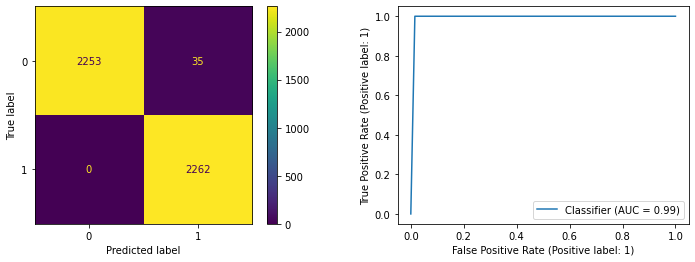
\includegraphics[scale=0.6]{knn}

Готовый классификатор {\tt KNeighborsClassifier} показывает идентичные результаты.

Наивный байесовский классификатор реализован в двух вариантах. Для его работы необходимо знать распределения каждого признака для каждого класса а также вероятности самих классов. Первый вариант оценивает распределения признаков используя ядерную оценку плотности вероятности ({\tt scipy.stats.gaussian\_kde}).

\begin{lstlisting}[language=python, keepspaces=true]
class NaiveBayes(BaseEstimator, ClassifierMixin):
    def __init__(self):
        pass
    
    def fit(self, data, labels):
        self.data = data
        self.labels = labels
        self.kde = []
        for c, count in zip(*np.unique(labels, return_counts=True)):
            self.kde.append([])
            for i in range(data.shape[1]):
                self.kde[-1].append(gaussian_kde(data[labels == c, i]))
        self.classes = np.unique(labels, return_counts=True)[1] / len(labels)
        return self
    
    def predict(self, data):
        res = np.ndarray((data.shape[0],))
        for i, obj in enumerate(data):
            prob = np.array(self.classes)
            for j in range(len(self.classes)):
                for k, kde in enumerate(self.kde[j]):
                    prob[j] *= kde(obj[k])[0]
            res[i] = prob.argmax()
        return res
\end{lstlisting}

Никаких параметров нет, в кросс-валидации нет необходимости. Результаты модели:

\begin{lstlisting}[frame=none, numbers=none]
Accuracy: 0.9345054945054945
Precision: 0.9593077642656689
Recall: 0.9067197170645447
\end{lstlisting}
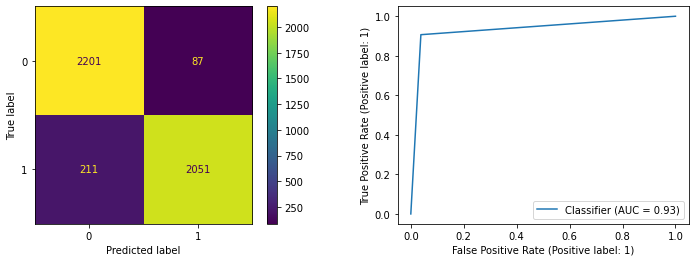
\includegraphics[scale=0.6]{naive_bayes}

Второй вариант исходит из предположения, что признаки распределены нормально. Соответственно, для каждого признака для каждого класса необходимо посчитать выборочное математическое ожидание и выборочную дисперсию, а при предсказании использовать формулу плотности вероятности нормального распределения.

\begin{lstlisting}[language=python, keepspaces=true]
class GaussianNaiveBayes(BaseEstimator, ClassifierMixin):
    def __init__(self):
        pass
    
    def fit(self, data, labels):
        self.data = data
        self.labels = labels
        self.means = []
        self.stds = []
        for c in np.unique(labels):
            self.means.append(data[labels == c,].mean(axis=0))
            self.stds.append(data[labels == c,].std(axis=0))
        self.classes = np.unique(labels, return_counts=True)[1] / len(labels)
        return self
    
    def predict(self, data):
        res = np.ndarray((data.shape[0],))
        for i, obj in enumerate(data):
            prob = np.array(self.classes)
            for j in range(len(self.classes)):
                prob[j] *= np.cumprod(1 / self.stds[j] / np.sqrt(2 * np.pi) * 
                                      np.exp(((obj - self.means[j]) / self.stds[j]) ** 2 / -2))[-1]
            res[i] = prob.argmax()
        return res
\end{lstlisting}

Результаты:

\begin{lstlisting}[frame=none, numbers=none]
Accuracy: 0.9125274725274726
Precision: 0.9375586854460094
Recall: 0.8828470380194519
\end{lstlisting}
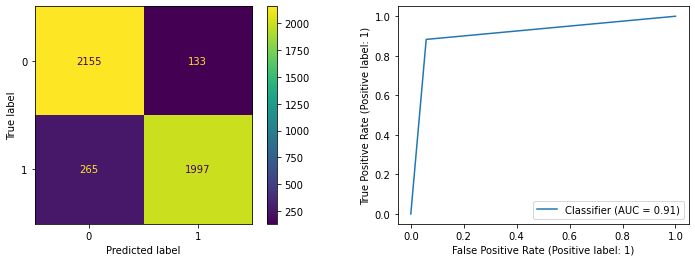
\includegraphics[scale=0.6]{gauss_naive_bayes}

Видно, что предположение о гауссовости приводит к несколько более худшим результатам. Рассмотрим распределения признаков в обоих случаях:

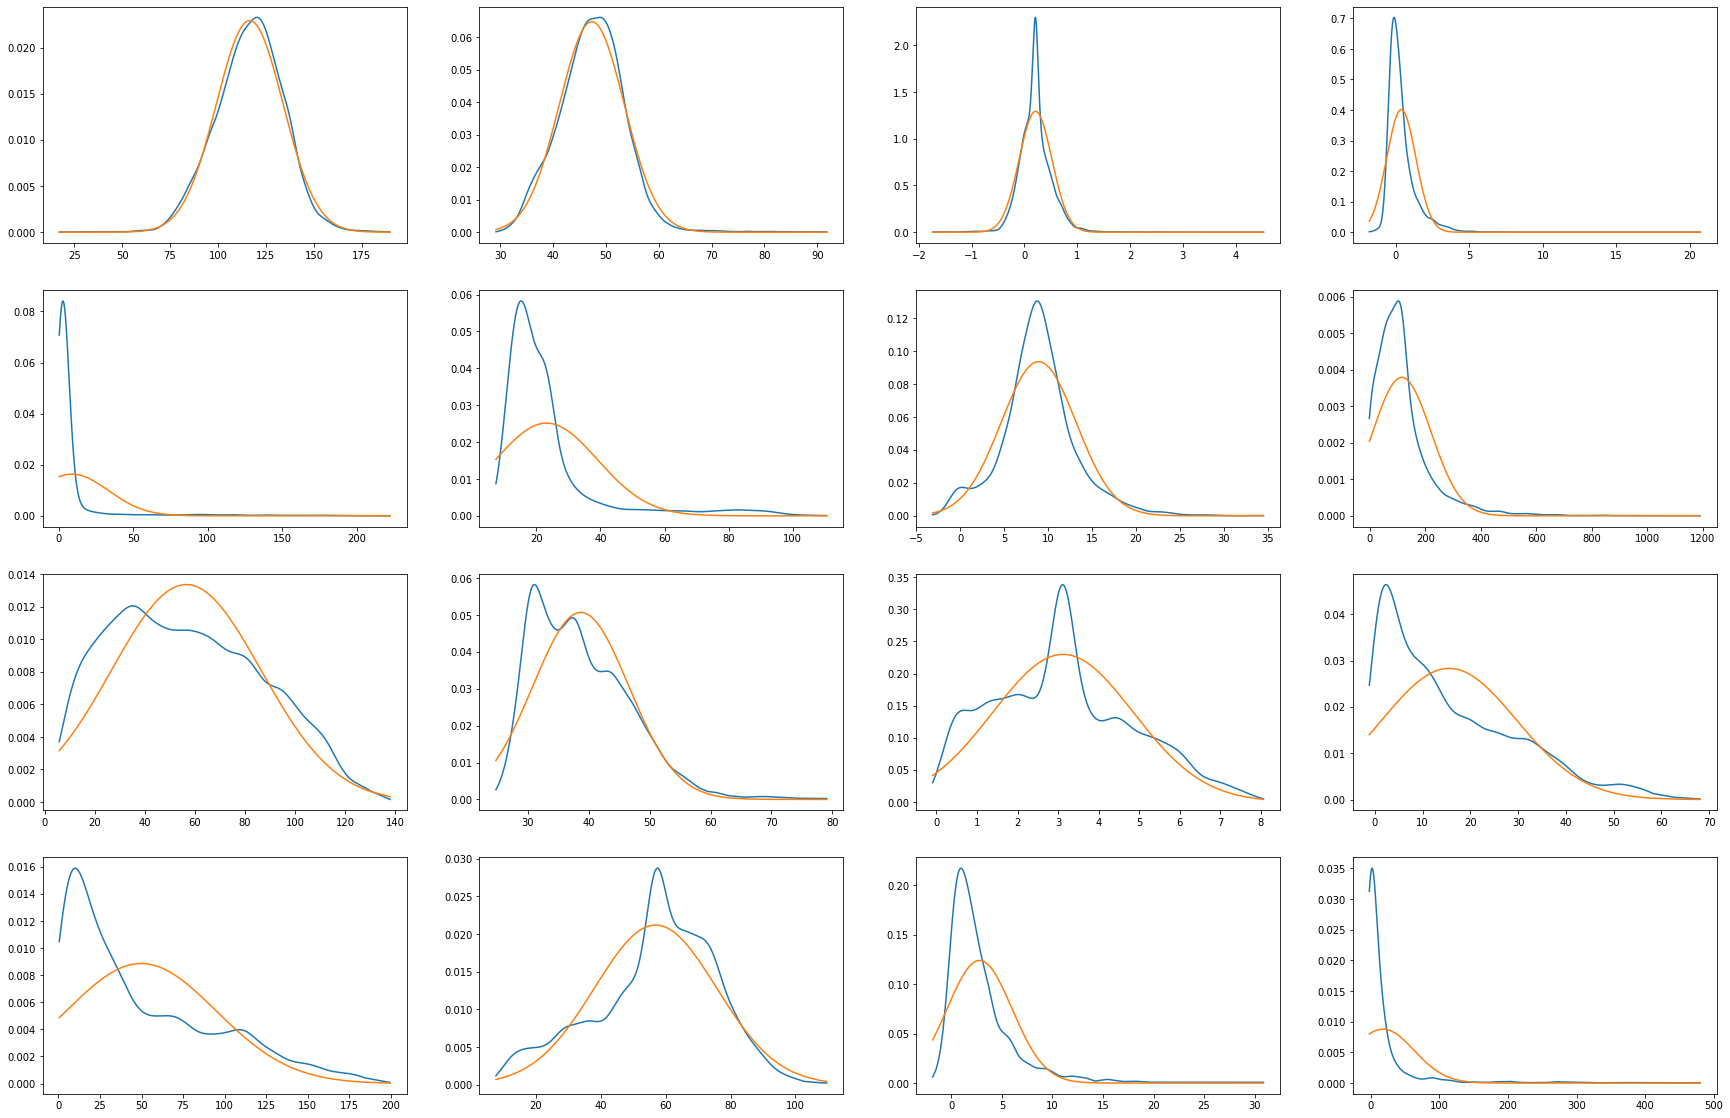
\includegraphics[width=\textwidth]{features}

Из графиков следует, что, тогда как распределение некоторых признаков довольно хорошо аппроксимируется нормальным, другие имеют более сложную структуру, что и приводит к разнице в результатах. Из преимуществ второго подхода можно отметить более высокую скорость работы и меньшие затраты памяти.

Готовый классификатор {\tt GaussianNB} показывает результаты, идентичные второй реализации.

Логистическая регрессия проводит разделяющую гиперплоскость в пространстве признаков. Для единообразия параметр смещения входит в вектор коэффициентов, при этом данные надо дополнить фиктивным признаком, всегда равным единице. Функция потерь имеет вид (с учетом $L_2$ регуляризации):
$$L(w, X, y) = \alpha\|w\|^2_2 - \sum_i \big( y_i \log(\sigma(\langle w, x_i \rangle)) + (1 - y_i) \log(\sigma(-\langle w, x_i \rangle)) \big)$$
где $\sigma(z) = \frac1{1 + e^{-z}}$ --- сигмоида. Градиент функции потерь:
$$\nabla_w L(y, X, w) = 2 \alpha w - \sum_i x_i \big( y_i - \sigma(\langle w, x_i \rangle)) \big)$$
Для минимизации функции потерь используем стохастический градиентный спуск, размер минибатча и число эпох --- гиперпараметры. Итого, вместе с темпом обучения и множителем регуляризации --- четыре гиперпараметра.

\begin{lstlisting}[language=python, keepspaces=true]
class LogisticRegression(BaseEstimator, ClassifierMixin):
    def __init__(self, lr=0.1, batch=10, epochs=1, alpha=0.0001):
        self.lr = lr
        self.batch = batch
        self.epochs = epochs
        self.alpha = alpha
    
    def fit(self, data, labels):
        self.w = np.random.normal(0, 1, (data.shape[1]+1,))
        data = np.concatenate((data, np.ones((data.shape[0],1))), axis=1)
        for _ in range(self.epochs):
            for i in range(self.batch, len(data), self.batch):
                data_batch = data[i-self.batch:i]
                labels_batch = labels[i-self.batch:i]
                
                pred = self.sigmoid(np.dot(self.w, data_batch.T))
                grad = 2 * self.alpha * self.w + np.dot(pred - labels_batch, data_batch)
                
                self.w -= self.lr * grad
        return self
    
    def sigmoid(self, x):
        return 1 / (1 + np.exp(-x))
    
    def predict(self, data):
        return (self.sigmoid(np.concatenate((data, np.ones((data.shape[0],1))), axis=1).dot(self.w)) > 0.5).astype('int64')
\end{lstlisting}

Так как параметров стало больше, для кросс-валидации используем и поиск по сетке и случайный поиск. Случайный поиск быстрее сходится, но не обязательно приводит к глобальному максимуму. Поиск по сетке дает лучшие результаты, но намного медленнее работает. Также логистическая регрессия нуждается в нормализации данных. Оптимальные параметры модели:

\begin{lstlisting}[frame=none, numbers=none]
lr: 0.1
alpha: 0.0001
batch: 100
epochs: 100
\end{lstlisting}

Результаты модели:

\begin{lstlisting}[frame=none, numbers=none]
Accuracy: 0.9345054945054945
Precision: 0.9716618635926993
Recall: 0.8943412908930151
\end{lstlisting}
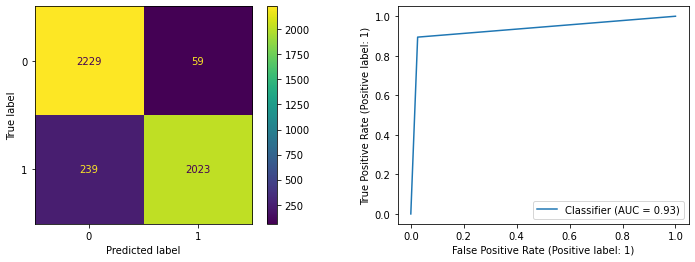
\includegraphics[scale=0.6]{log_regr}

Готовый классификатор {\tt SGDClassifier(loss='log')} по неизвестным причинам хуже на несколько процентов.

Метод опорных векторов аналогичен регрессии, за исключением цели оптимизации. Здесь это максимизация расстояния от гиперплоскости до разделяемых объектов. Его функция потерь имеет вид (с учетом $L_2$ регуляризации):
$$L(w, x, y) = \alpha\|w\|^2_2 + \sum_i \max(0, 1-y_i \langle w, x_i\rangle)$$
Ее градиент:
\begin{equation*}
\nabla_w L(w, x, y) = 2 \alpha w + \sum_i
\begin{cases} 
    0,           & 1 - y_i \langle w, x_i \rangle \leq 0 \\
    - y_i x_i,   & 1 - y_i \langle w, x_i \rangle > 0
\end{cases}
\end{equation*}
Модель имеет те же четыре гиперпараметра.

\begin{lstlisting}[language=python, keepspaces=true]
class SVM(BaseEstimator, ClassifierMixin):
    def __init__(self, lr=0.1, batch=10, epochs=1, alpha=0.0001):
        self.lr = lr
        self.batch = batch
        self.epochs = epochs
        self.alpha = alpha
    
    def fit(self, data, labels):
        self.w = np.random.normal(0, 1, (data.shape[1]+1,))
        data = np.concatenate((data, np.ones((data.shape[0],1))), axis=1)
        labels = labels * 2 - 1
        for _ in range(self.epochs):
            for i in range(self.batch, len(data), self.batch):
                data_batch = data[i-self.batch:i]
                labels_batch = labels[i-self.batch:i]
                
                grad = 2 * self.alpha * self.w
                for i, x in enumerate(data_batch):
                    if 1 - x.dot(self.w) * labels_batch[i] > 0:
                        grad -= x * labels_batch[i]
                
                self.w -= self.lr * grad
        return self

    def predict(self, data):
        return (np.sign(np.concatenate((data, np.ones((data.shape[0],1))), axis=1).dot(self.w)) + 1) / 2
\end{lstlisting}

Оптимальные параметры модели:

\begin{lstlisting}[frame=none, numbers=none]
lr: 0.01
alpha: 0.001
batch: 100
epochs: 100
\end{lstlisting}

Результаты модели:

\begin{lstlisting}[frame=none, numbers=none]
Accuracy: 0.9547252747252747
Precision: 0.978584729981378
Recall: 0.9292661361626879
\end{lstlisting}
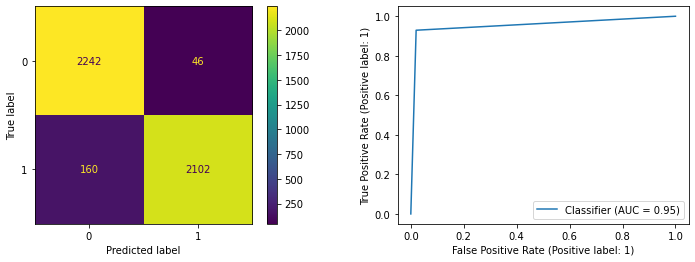
\includegraphics[scale=0.6]{svm}

Готовый классификатор {\tt SGDClassifier(loss='hinge')} аналогично хуже на несколько процентов.

\pagebreak

